\documentclass[]{article}

\usepackage{graphicx}
\usepackage{amsmath}
\usepackage[margin=1.0in]{geometry}

%opening
\title{Ranking Answers and Web Passages for Non-factoid Question Answering: Emory University at TREC LiveQA}
\author{Denis Savenkov\\Emory University\\dsavenk@emory.edu}
\date{}

\begin{document}

\maketitle

\begin{abstract}
This paper describes a question answering system built by a team from Emory University to participate in TREC LiveQA shared task.
The system is based on a single trained model, that ranks candidate answers extracted from two different sources: answers to similar questions previously posted to Yahoo! Answers community question answering (CQA) platform and passages from documents retrieved using Bing Web Search API.
The ranking model is trained on question and answer (QnA) pairs from Yahoo! Answers WebScope dataset\footnote{https://webscope.sandbox.yahoo.com/catalog.php?datatype=l} using pairwise ranking criteria.
The features used for ranking includes statistics over the candidate answer text, lexicalized features of term pairs from question and answer texts, information about matched terms, Okapi BM25 retrieval score and the output produced by a Long Short-Term Memory (LSTM) neural network model.
The system performed above average on most of the evaluation metrics.

\end{abstract}

\section{Introduction}
% This paragraph can probably be removed, too general.
Over the years of question answering research the focus was mainly around factoid questions, which constitute only a small part of user information needs.
Factoid questions are usually defined as those that can be answered with a short phrase, which is often a number or a named entity.
Causation, manner, reason, opinion, advice and other similar types of questions are beyond the scope of the factoid question answering systems.
One way to solve these questions is to ask other people, and community question answering websites (e.g. Yahoo! Answers\footnote{http://answers.yahoo.com/}, Answer.com, StackExchange.com, etc.) became very popular and currently contain millions of questions and answers.
This year TREC pioneered a LiveQA shared task, which targets automatic answering of questions posted to Yahoo! Answers CQA website.
This was author's first attempt in question answering and I decided to implement a relatively simple model as a baseline that can be improved upon next year should TREC LiveQA be offered again.

There are a lot of different types of questions that users post to CQA websites and it is probably beneficial to study them separately.
However, for simplicity the model I built treats all questions in the same way.
The idea is to have a single model, that ranks a set of extracted answer candidates.
The system doesn't try to identify if candidates match the question and simply returns the highest ranked candidate as the answer.
Preliminary analysis of questions and potential answer sources gave an insight that the best data source is answers to similar questions in case we are able to find any.
People often have similar tasks and situations which pose same questions.
Therefore, it's frequently the case that a similar question was already asked by someone and potentially even received a good reply and can be reused to answer new questions \cite{Shtok:2012:LPA:2187836.2187939}.
Of course, many questions are indeed unique or contain unique details, which makes it impossible to find a good match from the existing answers.
Therefore I retract to web search to generate additional answer candidates.
For non-factoid questions it's harder to use the redundancy of the information on the web, which is exploited very effectively in factoid QA \cite{Lin:2007:EPU:1229179.1229180}.
The system I developed extracts passages containing question terms from all retrieved web documents independently.
For training I used the publicly available collection of QnA pairs from Yahoo! Answers.
The assumption made was that for each question the answer selected as the ``best answer'' on Yahoo! Answers is indeed the best and should be ranked higher than answers to other questions.
However, taking all other answers is intractable and probably detrimental as almost all of them would be totally unrelated to the subject of the given question.
Therefore, I used search to retrieve a set of similar questions and took their answers as negative examples.
The following chapters describe the QA system in more details.

\section{Approach}

\begin{figure}
	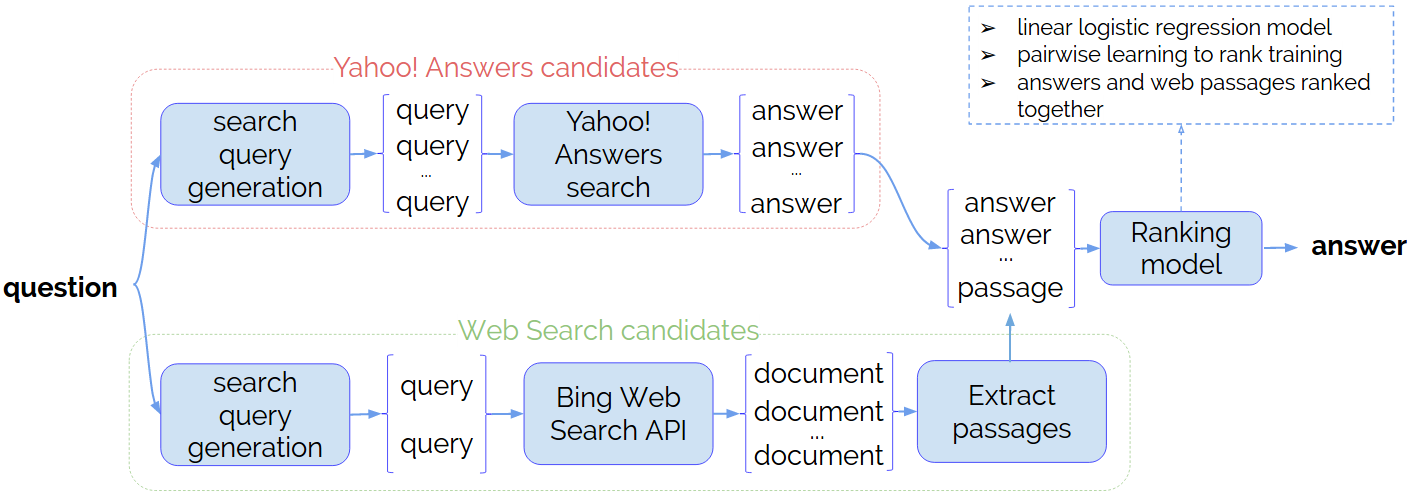
\includegraphics[width=460px]{img/qa_model}
	\caption{Architecture of our question answering system}
	\label{figure:qa_model}
\end{figure}

The general architecture of our question answering system is presented on Figure \ref{figure:qa_model}.
It uses two primary data sources for generating answer candidates: answers to similar questions from Yahoo! Answers website and documents retrieved using web search. 
All candidates are mixed together, ranked and the top answer is returned.

\subsection{Candidate generation}
 
Each question issued to a QA system in TREC LiveQA consists of 3 main parts: title, body and category.
For example:

\vspace{0.3cm}
\begin{tabular}{|p{15cm}|}
\hline
\textbf{Question category}: Astronomy \& Space\\
\textbf{Question title}: Why do people claim the Earth isn't the center of the universe?\\
\textbf{Question body}: Clearly the sun and moon are moving around the Earth otherwise we wouldn't have night and day.\\
\hline
\end{tabular}
\vspace{0.3cm}

When the QA system receives a question it first generates a set of candidate answers from Yahoo! Answers and regular web search.
To generate a set of candidates the system produces one or more search queries and issues them to both resources.

To find similar questions and extract the corresponding answers from Yahoo! Answers we use the search functionality already available on the website.
Some questions are very concise while other provide many useful as well as redundant details.
Ideally we want to match as many of them as possible, however, there is a chance that search won't return any results if there are no good matches.
Therefore the system generates a set of search queries of various details level, issues them all to Yahoo! Answers search and collects top 10 responses from all of them.
Here is the list of queries that our system generates:
\begin{itemize}
	\setlength\itemsep{0mm}
	\item Concatenation of question title and question body (with and without stopwords)
	\item Question title only (with and without stopwords)
	\item Question title concatenated with question body and question category
	\item Question title concatenated with the name of the question category
	\item Top 5 terms from question title scored by tf-idf\footnote{Document frequency is computed on WebScope collection of QnA pairs from Yahoo! Answers}
	\item Top 5 terms from question title and body scored by tf-idf
\end{itemize}

For each query and top-10 retrieved questions the system extracts its top answer if provided and puts it into the candidate pool along with some information about the corresponding question and its category.

To extract candidate passages from relevant web documents previous research in factoid question answering have tried query reformulations \cite{Agichtein:2001:LSE:371920.371976} to better match the potential answer text.
However recently \cite{askmsr_plus15} demonstrated that such reformulations are no longer necessary as search engines have improved the query processing techniques.
Inspired by this observation and considering that retrieving web documents and extracting passages from them is more time consuming, the system issues only 2 web search queries: question title and title concatenated with body. 
We use Bing Web Search API\footnote{http://datamarket.azure.com/dataset/bing/searchweb} and the system downloads top-10 retrieved documents, parses HTML code and extracts the main content text \cite{Kohlschutter_2010}.
Document content is further split into sentences \cite{manning2014stanford} and candidates are built by taking contiguous sequence of sentences no longer than the answer character limit\footnote{In the final run the limit was 1000 characters}.
The model only keeps passages that contain at least one non-stopword from the question.
Snippet generated by Bing and included in search results returned by the API is also added as one of the candidates.

\subsection{Candidate ranking}

A trained linear logistic regression model is used to rank candidate answers, represented with a set of features:
\begin{itemize}
\setlength\itemsep{0mm}
\item answer text statistics: length in character, tokens and sentences, average number of tokens per sentence.
\item Okapi BM25 scores, which consider question title and concatenation of title and body as queries. Term statistics were computed on Yahoo! Answers WebScope dataset. The score is calculated as follows:
\begin{equation*}
\label{equation:bm25}
\text{score}(A,Q) = \sum_{i=1}^{n} \text{IDF}(q_i) \cdot \frac{f(q_i, A) \cdot (k_1 + 1)}{f(q_i, A) + k_1 \cdot (1 - b + b \cdot \frac{|A|}{\text{avg\_al}})}
\end{equation*}
where $f(q_i, A)$ is frequency of term $q_i$ in the answer text, $k_1=1.2$, $B=0.75$ and $avg_al=50$ (average answer length).
\item term matches features: lemmas, part of speech tags of matched terms between the question and answer texts, the fraction of unique question terms matched in the answer, length of the maximum span of matched terms in the answer.
\item number of matched terms between the question title, body and the title of the page from which the candidate answer is retrieved. For Yahoo! Answers the text of the retrieved question is used as title.
\item category match feature for Yahoo! Answers candidates.
\item pairs of lemmas from question and answer texts, that are supposed to bridge the lexical gap between question and answer language.
\item average, minimum and maximum normalized pointwise mutual information (NPMI) scores between pairs of terms from the question and answer texts. The scores are estimated from QnA pairs from Yahoo! Answers WebScope dataset using the following formula:
\begin{equation*}
\begin{split}
\operatorname{npmi}(q_i;a_j) = \frac{pmi(q_i;a_j)}{-\log p(q_i,a_j)}\\
\operatorname{pmi}(q_i;a_j) = \log\frac{p(q_i,a_j)}{p(q_i)p(a_j)} =  \log\frac{p(a_j|q_i)}{p(a_j)}
\end{split}
\end{equation*}
\item QnA pair score from a Long Short Term Memory (LSTM) neural network model, described in Section \ref{section:lstm}.
\end{itemize}

The candidate with the highest score is returned as the answer to the question.
If something goes wrong and no candidates were generated or some problem occurred the system returns ``I don't know'' as the default answer.

\subsection{Model Training}

There are two trained models used in the system: LSTM recurrent neural network based model, which is used as one of the features for the final logistic regression model that scores all candidates and selects the best one as the answer.

\subsubsection{LSTM model}
\label{section:lstm}

Deep learning models have a huge success in image and speech problems and shows some very promising results in natural language processing and question answering, e.g. \cite{yu2014deep,diwang_lstm_2015} to name a few.
I decided to explore this direction and built a recurrent neural network model to score how well does a candidate answer a question.
Long Short-Term Memory (LSTM) \cite{hochreiter1997long} is a particular architecture of recurrent neural networks that allows to reduce exploding and vanishing gradients problems.
The model I developed reads question and answer tokens and produces a probability score based on a vector representation of a QnA pair.
Figure \ref{figure:lstm_model} shows a structure of the model.

\begin{figure}
	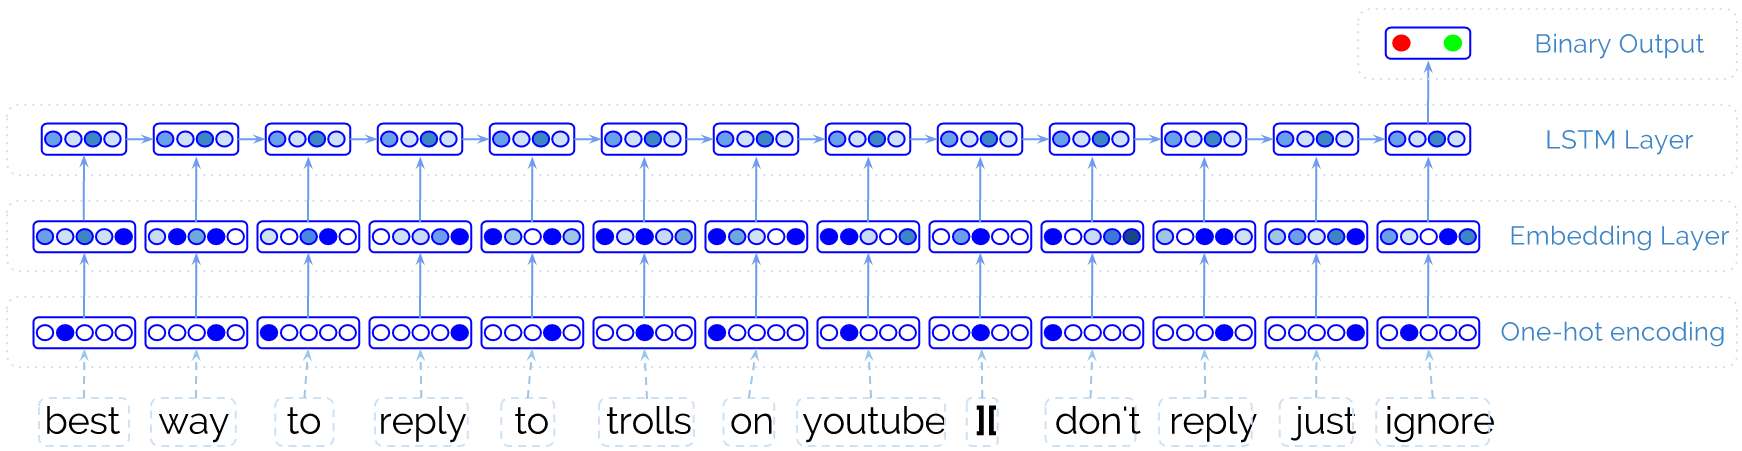
\includegraphics[width=470px]{img/qa_lstm}
	\caption{LSTM model for answer scoring. The example shows a QnA pair where the question is ``Best way to reply to trolls on youtube?'' and the answer is ``Don't reply, just ignore''.}
	\label{figure:lstm_model}
\end{figure}

Question (title with body) and answer texts are tokenized, punctuation characters are removed and for each token lowercase lemma is taken.
The sequences are limited to 100 elements and concatenated through a sentinel separator character so the model knows where the question the answer starts.
The hidden state of the model after the whole sequence is processed is used by logistic regression unit to output a probability, that the candidate answers the question well.

To train the model QnA pairs from Yahoo! Answers WebScope dataset were used (we selected a subset of questions from the categories chosen for TREC LiveQA).
Each question and the corresponding best answer was used as a positive training example.
To generate negative examples I didn't take random example as they will be totally unrelated, and instead took answers to similar questions.
All questions were indexed with Lucene library and similar questions were retrieved using built-in BM25 retrieval model.
For each question and correct answer pair from the dataset 10 similar questions were retrieved and the corresponding answers were used as negative examples for training\footnote{It's true, that some of them can indeed be relevant to the original question}.

The model was implemented using Keras\footnote{http://keras.io} library.
We used an embedding and hidden layers of dimension 128 and the vocabulary size of 1M words (we used hashing to generate word ids).
The model was trained using Adam optimization technique \cite{kingma2014adam} with mini batches of size 200 instances for 100 epochs.

\subsubsection{Logistic regression model}

The final model that ranks all answer candidates is a linear L2-regularized logistic regression model.
To train the model we also use QnA pairs from Yahoo! Answers WebScope dataset, although different splits are used to train LSTM and logistic regression models.
For each question the corresponding ``best answer'' is taken as the correct one.
To get a sample of negative examples Lucene index is used again and answers to 10 most similar questions are retrieved.
Different from LSTM model training, here I took a pairwise approach for learning to rank and generated a training examples from pairs of different answers to the same question, where one answer is the correct one.
That is, let the current question be $Q$, its ``correct'' answer $A^*$, and retrieved candidates $A_1, ..., A_n$.
Each candidate is represented with a set of features: $f(Q, A^*)$, $f(Q, A_1)$, ..., $f(Q, A_n)$.
For each $i=1..n$ we create two training instances, i.e. class 1: $\langle A^*, A_i\rangle$ and class -1: $\langle A_i, A^*\rangle$.
Each such instance is represented with pairwise differences of answer features, e.g. $\langle A^*, A_i\rangle: f_{pair}(Q, \langle A^*, A_i\rangle) = f(Q, A^*) - f(Q, A_i)$.
Since the trained model is linear, therefore if $w(f(Q, A^*) - f(Q, A_i)) > 0$ then $w f(Q, A^*) > w f(Q, A_i)$ and we can rank candidates by the score produced by the model, i.e. $w f(Q, A_i)$.

\section{Results and Analysis}

From the final run of the system, 1087 questions were judged by the organizers on a scale from 1 to 4:\\
\textbf{4: Excellent} - a significant amount of useful information, fully answers the question\\
\textbf{3: Good} - partially answers the question\\
\textbf{2: Fair} - marginally useful information\\
\textbf{1: Bad} – contains no useful information for the question\\
\textbf{-2}: the answer is unreadable  (only 15 answers from all runs were judged as unreadable)

The following performance metrics were reported:
\begin{itemize}
\setlength\itemsep{0mm}
\item \textbf{avg-score(0-3)}: average score over all questions, where scores are translated to 0-3 range. This metric considers ``Bad'', unreadable answers and unanswered questions as having score 0
\item \textbf{succ@i+}: the fraction of answers with score i or greater (i=1..4)
\item \textbf{prec@i+}: the number of questions with score i or greater (i=2..4) divided by the number of answered questions
\end{itemize}
Table \ref{table:liveqa-results} provides the official results of our run and average scores over all runs.

\begin{table}
\caption{Results of the TREC LiveQA evaluation of Emory University QA system and average results of all systems. $\uparrow$ means that results of Emory system in this metric are above average, and $\downarrow$ means that results are below average}
\label{table:liveqa-results}
\begin{tabular}{|p{2cm}|p{1.4cm}|p{1.3cm}|p{1.3cm}|p{1.3cm}|p{1.3cm}|p{1.3cm}|p{1.3cm}|p{1.3cm}|}
\hline
 & avg score (0-3) & succ@1+ & succ@2+ & succ@3+ & succ@4+ & prec@2+ &
 prec@3+ & prec@4+ \\
\hline
Average of all runs & 0.465 & 0.925 & 0.262 & 0.146 & 0.060 & 0.284 & 0.159 & 0.065\\
 \hline
Emory run & 0.605 $\uparrow$ & 0.812 $\downarrow$ & 0.332 $\uparrow$ & 0.190 $\uparrow$ & 0.086 $\uparrow$ & 0.408 $\uparrow$ & 0.233 $\uparrow$ & 0.106 $\uparrow$\\
\hline
\end{tabular}
\end{table}

As we can see from Table \ref{table:liveqa-results} for most of the metrics except succ@1+ results of our run is above average.
The metric succ@1+ shows the fraction of questions for which a readable answer was returned by the system.
A lower score in this metic means that my system didn't return an answer in time in almost 20 \% of the cases.
A part of the problem is caused by several technical issues, that appeared on the day of the evaluation run.
Due to one of them LSTM model didn't provide any score for a significant fraction of submitted questions, and the other problem made the whole system unresponsive for a couple of hours.
Nevertheless, the overall results look promising and I will make a more thorough analysis of the system performance for the final version of the paper.

The absolute values of the performance metrics demonstrate a great room for improvement as our system was able to return partial or good answer only in 23\% of the cases (prec@3+) when the answer was returned.
And for 60\% of the questions the answer doesn't contain any useful information.

%\section{Conclusion}
%TREC LiveQA is a very exciting task, which will trigger an advancement of question answering state-of-the-art beyond the factoid questions.
%I've enjoyed working on the task and hope to see the next version in the upcoming year.
%The developed system performance is a good baseline, which showed how difficult it is to find good answers for non-factoid questions.


\bibliographystyle{unsrt}
\bibliography{bibliography.bib}

\end{document}
